\definecolor{aa}{RGB}{200,200,200}
\definecolor{ab}{RGB}{161,218,180}
\definecolor{ac}{RGB}{65,182,196}
\definecolor{ad}{RGB}{44,127,184}

% GNUPLOT: LaTeX picture with Postscript
\begingroup
  \makeatletter
  \providecommand\color[2][]{%
    \GenericError{(gnuplot) \space\space\space\@spaces}{%
      Package color not loaded in conjunction with
      terminal option `colourtext'%
    }{See the gnuplot documentation for explanation.%
    }{Either use 'blacktext' in gnuplot or load the package
      color.sty in LaTeX.}%
    \renewcommand\color[2][]{}%
  }%
  \providecommand\includegraphics[2][]{%
    \GenericError{(gnuplot) \space\space\space\@spaces}{%
      Package graphicx or graphics not loaded%
    }{See the gnuplot documentation for explanation.%
    }{The gnuplot epslatex terminal needs graphicx.sty or graphics.sty.}%
    \renewcommand\includegraphics[2][]{}%
  }%
  \providecommand\rotatebox[2]{#2}%
  \@ifundefined{ifGPcolor}{%
    \newif\ifGPcolor
    \GPcolorfalse
  }{}%
  \@ifundefined{ifGPblacktext}{%
    \newif\ifGPblacktext
    \GPblacktexttrue
  }{}%
  % define a \g@addto@macro without @ in the name:
  \let\gplgaddtomacro\g@addto@macro
  % define empty templates for all commands taking text:
  \gdef\gplfronttext{}%
  \gdef\gplfronttext{}%
  \makeatother
  \ifGPblacktext
    % no textcolor at all
    \def\colorrgb#1{}%
    \def\colorgray#1{}%
  \else
    % gray or color?
    \ifGPcolor
      \def\colorrgb#1{\color[rgb]{#1}}%
      \def\colorgray#1{\color[gray]{#1}}%
      \expandafter\def\csname LTw\endcsname{\color{white}}%
      \expandafter\def\csname LTb\endcsname{\color{black}}%
      \expandafter\def\csname LTa\endcsname{\color{black}}%
      \expandafter\def\csname LT0\endcsname{\color[rgb]{1,0,0}}%
      \expandafter\def\csname LT1\endcsname{\color[rgb]{0,1,0}}%
      \expandafter\def\csname LT2\endcsname{\color[rgb]{0,0,1}}%
      \expandafter\def\csname LT3\endcsname{\color[rgb]{1,0,1}}%
      \expandafter\def\csname LT4\endcsname{\color[rgb]{0,1,1}}%
      \expandafter\def\csname LT5\endcsname{\color[rgb]{1,1,0}}%
      \expandafter\def\csname LT6\endcsname{\color[rgb]{0,0,0}}%
      \expandafter\def\csname LT7\endcsname{\color[rgb]{1,0.3,0}}%
      \expandafter\def\csname LT8\endcsname{\color[rgb]{0.5,0.5,0.5}}%
    \else
      % gray
      \def\colorrgb#1{\color{black}}%
      \def\colorgray#1{\color[gray]{#1}}%
      \expandafter\def\csname LTw\endcsname{\color{white}}%
      \expandafter\def\csname LTb\endcsname{\color{black}}%
      \expandafter\def\csname LTa\endcsname{\color{black}}%
      \expandafter\def\csname LT0\endcsname{\color{black}}%
      \expandafter\def\csname LT1\endcsname{\color{black}}%
      \expandafter\def\csname LT2\endcsname{\color{black}}%
      \expandafter\def\csname LT3\endcsname{\color{black}}%
      \expandafter\def\csname LT4\endcsname{\color{black}}%
      \expandafter\def\csname LT5\endcsname{\color{black}}%
      \expandafter\def\csname LT6\endcsname{\color{black}}%
      \expandafter\def\csname LT7\endcsname{\color{black}}%
      \expandafter\def\csname LT8\endcsname{\color{black}}%
    \fi
  \fi
    \setlength{\unitlength}{0.0500bp}%
    \ifx\gptboxheight\undefined%
      \newlength{\gptboxheight}%
      \newlength{\gptboxwidth}%
      \newsavebox{\gptboxtext}%
    \fi%
    \setlength{\fboxrule}{0.5pt}%
    \setlength{\fboxsep}{1pt}%
\begin{picture}(6000.00,2400.00)%
    \gplgaddtomacro\gplfronttext{%
      \colorrgb{0.15,0.15,0.15}%
      \put(648,264){\makebox(0,0)[r]{\strut{}$0.000$}}%
      \colorrgb{0.15,0.15,0.15}%
      \put(648,655){\makebox(0,0)[r]{\strut{}$0.002$}}%
      \colorrgb{0.15,0.15,0.15}%
      \put(648,1046){\makebox(0,0)[r]{\strut{}$0.004$}}%
      \colorrgb{0.15,0.15,0.15}%
      \put(648,1437){\makebox(0,0)[r]{\strut{}$0.006$}}%
      \colorrgb{0.15,0.15,0.15}%
      \put(648,1828){\makebox(0,0)[r]{\strut{}$0.008$}}%
      \colorrgb{0.15,0.15,0.15}%
      \put(648,2219){\makebox(0,0)[r]{\strut{}$0.010$}}%
      \colorrgb{0.15,0.15,0.15}%
      \put(890,44){\makebox(0,0){\strut{}$0.01$}}%
      \colorrgb{0.15,0.15,0.15}%
      \put(1438,44){\makebox(0,0){\strut{}$0.03$}}%
      \colorrgb{0.15,0.15,0.15}%
      \put(1986,44){\makebox(0,0){\strut{}$0.05$}}%
      \colorrgb{0.15,0.15,0.15}%
      \put(2534,44){\makebox(0,0){\strut{}$0.10$}}%

      \put(3100,3139){\makebox(0,0){\strut{}Μέσο σφάλμα προσανατολισμού [rad], $\overline{\delta}_\theta = \pi$ rad}}
      \put(1850,2739){\makebox(0,0){\strut{}{$\small N_s$ \color{aa}{\rule[0.6mm]{0.5cm}{0.5mm}}}\footnotesize $360$}}
      \put(2650,2739){\makebox(0,0){\strut{}{\color{ab}{\rule[0.6mm]{0.5cm}{0.5mm}}}\footnotesize $720$}}
      \put(3350,2739){\makebox(0,0){\strut{}{\color{ac}{\rule[0.6mm]{0.5cm}{0.5mm}}}\footnotesize $1440$}}
      \put(4150,2739){\makebox(0,0){\strut{}{\color{ad}{\rule[0.6mm]{0.5cm}{0.5mm}}}\footnotesize $2880$}}

      \put(1700,2439){\makebox(0,0){\strut{}$\sigma_{\bm{M}} = 0.0$ m}}
      \put(4500,2439){\makebox(0,0){\strut{}$\sigma_{\bm{M}} = 0.05$ m}}
    }%
    \gplgaddtomacro\gplfronttext{%
    }%
    \gplgaddtomacro\gplfronttext{%
      \colorrgb{0.15,0.15,0.15}%
      \put(3432,264){\makebox(0,0)[r]{\strut{}$0.025$}}%
      \colorrgb{0.15,0.15,0.15}%
      \put(3432,1046){\makebox(0,0)[r]{\strut{}$0.026$}}%
      \colorrgb{0.15,0.15,0.15}%
      \put(3432,1828){\makebox(0,0)[r]{\strut{}$0.027$}}%
      \colorrgb{0.15,0.15,0.15}%
      \put(3674,44){\makebox(0,0){\strut{}$0.01$}}%
      \colorrgb{0.15,0.15,0.15}%
      \put(4222,44){\makebox(0,0){\strut{}$0.03$}}%
      \colorrgb{0.15,0.15,0.15}%
      \put(4771,44){\makebox(0,0){\strut{}$0.05$}}%
      \colorrgb{0.15,0.15,0.15}%
      \put(5319,44){\makebox(0,0){\strut{}$0.10$}}%
    }%
    \gplgaddtomacro\gplfronttext{%
      \colorrgb{0.15,0.15,0.15}%
      \put(3100,-359){\makebox(0,0){\strut{}Τυπική απόκλιση των διαταραχών του $\mathcal{S}_R$, $\sigma_R$ [m]}}%
      \colorrgb{0.00,0.00,0.00}%
      %\put(4496,2439){\makebox(0,0){\strut{}title}}%
    }%
    \put(0,0){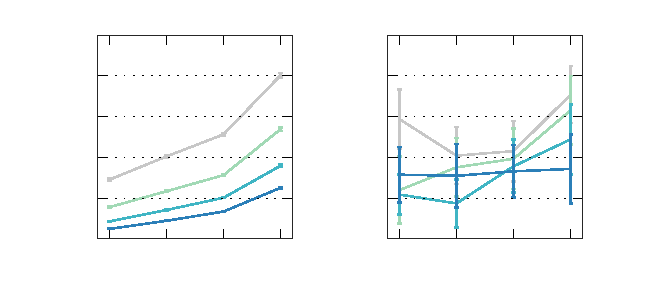
\includegraphics{./figures/parts/02/chapters/04/sections/02/errorbar_x1}}%
    \gplfronttext
  \end{picture}%
\endgroup
